% Editable vector figures used throughout the notes.

\newcommand{\TrainingPipelineFigure}{%
\begin{figure}[htbp]
\centering
\begin{tikzpicture}[
  box/.style={draw=Blue,rounded corners,fill=PaleBlue,align=center,minimum height=9mm,inner xsep=3mm,font=\scriptsize},
  held/.style={draw=Orange,rounded corners,fill=PaleOrange,align=center,minimum height=9mm,inner xsep=3mm,font=\scriptsize},
  arr/.style={-{Latex[length=2.2mm]},thick,color=Ink!75}
]
\node[box] (data) at (0,0) {Raw data};
\node[box] (split) at (2.6,0) {Train--test split};
\node[box] (train) at (5.1,1.15) {Training set};
\node[box] (prep) at (8.2,1.15) {Fit preprocessing\\and candidate models\\inside validation/CV};
\node[box] (model) at (11.4,1.15) {Selected model};
\node[held] (test) at (6.5,-1.15) {Held-out test set};
\node[held] (report) at (11.4,-1.15) {Final evaluation};
\draw[arr] (data) -- (split);
\draw[arr] (split) -- (train);
\draw[arr] (train) -- (prep);
\draw[arr] (prep) -- (model);
\draw[arr] (split) -- (test);
\draw[arr] (model) -- (report);
\draw[arr] (test) -- (report);
\end{tikzpicture}
\caption{Information boundaries in a training workflow. Scaling, feature selection, and resampling are fitted only on training data or training folds. The test set is used once, after model selection.}
\label{fig:training-pipeline}
\end{figure}}

\newcommand{\KnnGeometryFigure}{%
\begin{figure}[htbp]
\centering
\begin{tikzpicture}[scale=0.9]
\draw[-{Latex[length=2mm]},color=Ink!70] (0,0) -- (7,0) node[right] {$x_1$};
\draw[-{Latex[length=2mm]},color=Ink!70] (0,0) -- (0,5) node[above] {$x_2$};
\foreach \p in {(1.0,1.1),(1.5,1.8),(2.0,1.2),(2.1,2.4),(2.7,1.7),(3.0,2.7)}
  \fill[Blue] \p circle (2.1pt);
\foreach \p in {(4.3,3.0),(4.8,3.8),(5.3,2.8),(5.8,3.7),(6.1,2.5),(5.2,4.4)}
  \draw[Red,thick] \p ++(-2.2pt,-2.2pt) -- ++(4.4pt,4.4pt) \p ++(-2.2pt,2.2pt) -- ++(4.4pt,-4.4pt);
\coordinate (q) at (3.55,2.45);
\draw[Teal,very thick] (q) circle (3pt);
\draw[Teal,dashed,thick] (q) circle (1.45cm);
\node[Teal] at (3.55,3.15) {query};
\node[font=\small,align=left] at (5.35,0.65) {Distance defines the neighbourhood;\\scaling can change its members.};
\end{tikzpicture}
\caption{KNN searches for $k$ observations around a query. The circle represents one neighbourhood under a chosen distance scale; neighbourhoods become sparse in high dimensions.}
\label{fig:knn-geometry}
\end{figure}}

\newcommand{\LinearMarginFigure}{%
\begin{figure}[htbp]
\centering
\begin{tikzpicture}[scale=0.9]
\draw[-{Latex[length=2mm]},color=Ink!70] (0,0) -- (7,0) node[right] {$x_1$};
\draw[-{Latex[length=2mm]},color=Ink!70] (0,0) -- (0,5) node[above] {$x_2$};
\foreach \p in {(1.0,1.0),(1.5,2.0),(2.0,1.4),(2.2,2.9),(2.7,2.2)}
  \fill[Blue] \p circle (2.2pt);
\foreach \p in {(4.3,2.2),(4.8,3.2),(5.2,1.7),(5.7,3.8),(6.1,2.7)}
  \draw[Red,thick] \p ++(-2.3pt,-2.3pt) -- ++(4.6pt,4.6pt) \p ++(-2.3pt,2.3pt) -- ++(4.6pt,-4.6pt);
\draw[Navy,very thick] (3.5,0.35) -- (3.5,4.65) node[above] {$\vect w^\top\vect x+b=0$};
\draw[Navy!60,dashed,thick] (2.7,0.35) -- (2.7,4.65);
\draw[Navy!60,dashed,thick] (4.3,0.35) -- (4.3,4.65);
\draw[<->,Orange,thick] (2.7,0.65) -- node[below,font=\small] {margin} (4.3,0.65);
\draw[Orange,thick] (2.7,2.2) circle (4.5pt);
\draw[Orange,thick] (4.3,2.2) circle (4.5pt);
\end{tikzpicture}
\caption{Logistic regression, the perceptron, and SVM use the same linear score $z=\vect w^\top\vect x+b$. SVM additionally chooses a boundary with maximum geometric margin.}
\label{fig:linear-margin}
\end{figure}}

\newcommand{\BiasVarianceFigure}{%
\begin{figure}[htbp]
\centering
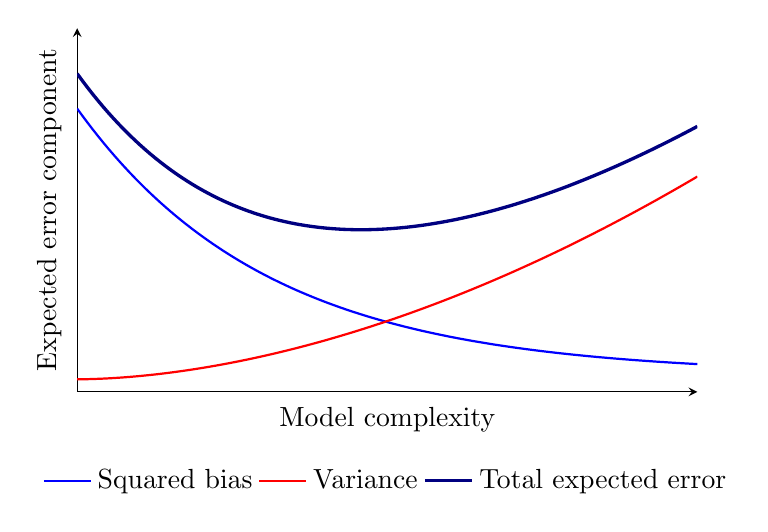
\begin{tikzpicture}
\begin{axis}[
  width=0.78\textwidth,height=6.2cm,
  axis lines=left,xlabel={Model complexity},ylabel={Expected error component},
  xmin=0,xmax=5,ymin=0,ymax=5.2,
  xtick=\empty,ytick=\empty,
  legend style={draw=none,fill=none,at={(0.5,-0.18)},anchor=north,legend columns=3},
  samples=120,domain=0:5
]
\addplot[Blue,thick] {3.8*exp(-0.65*x)+0.25};
\addlegendentry{Squared bias}
\addplot[Red,thick] {0.18+0.16*x^1.8};
\addlegendentry{Variance}
\addplot[Navy,very thick] {3.8*exp(-0.65*x)+0.16*x^1.8+0.75};
\addlegendentry{Total expected error}
\end{axis}
\end{tikzpicture}
\caption{As model complexity grows, bias often falls while variance rises. These curves describe a common pattern rather than a theorem for every model family; irreducible noise shifts the total error upward.}
\label{fig:bias-variance}
\end{figure}}

\newcommand{\PcaLdaFigure}{%
\begin{figure}[htbp]
\centering
\begin{tikzpicture}[scale=0.92]
\begin{scope}
\draw[-{Latex[length=2mm]},color=Ink!65] (0,0)--(5.7,0) node[right] {$x_1$};
\draw[-{Latex[length=2mm]},color=Ink!65] (0,0)--(0,4.2) node[above] {$x_2$};
\foreach \p in {(1.3,0.5),(1.8,1.2),(1.5,2.1),(1.9,3.1),(1.6,3.8)} \fill[Blue] \p circle (2pt);
\foreach \p in {(3.5,0.6),(3.9,1.3),(3.6,2.2),(4.0,3.0),(3.7,3.9)}
  \draw[Red,thick] \p ++(-2pt,-2pt)--++(4pt,4pt) \p ++(-2pt,2pt)--++(4pt,-4pt);
\draw[Teal,very thick,-{Latex[length=2.3mm]}] (2.65,0.35)--(2.65,3.95) node[above,font=\small] {PCA};
\draw[Orange,very thick,-{Latex[length=2.3mm]}] (0.75,2.15)--(4.75,2.15) node[right,font=\small] {LDA};
\end{scope}
\end{tikzpicture}
\caption{PCA selects directions of high total variance. LDA selects directions that maximise the ratio of between-class to within-class scatter. Their objectives are different.}
\label{fig:pca-lda}
\end{figure}}

\newcommand{\BackpropFigure}{%
\begin{figure}[htbp]
\centering
\begin{tikzpicture}[
  neuron/.style={circle,draw=Blue,fill=PaleBlue,minimum size=9mm,font=\small},
  loss/.style={rounded corners,draw=Orange,fill=PaleOrange,minimum height=9mm,inner xsep=3mm,font=\small},
  fwd/.style={-{Latex[length=2mm]},thick,color=Ink!70},
  bwd/.style={-{Latex[length=2mm]},thick,color=Red,dashed}
]
\node[neuron] (x1) at (0,1.2) {$x_1$};
\node[neuron] (x2) at (0,-1.2) {$x_2$};
\node[neuron] (h1) at (2.4,1.2) {$h_1$};
\node[neuron] (h2) at (2.4,-1.2) {$h_2$};
\node[neuron] (z) at (4.8,0) {$z$};
\node[loss] (l) at (7.0,0) {$L(y,\hat y)$};
\foreach \a in {x1,x2}\foreach \b in {h1,h2}\draw[fwd] (\a)--(\b);
\draw[fwd] (h1)--(z); \draw[fwd] (h2)--(z); \draw[fwd] (z)--(l);
\draw[bwd] (6.55,0.5) .. controls (5.9,1.15) and (5.2,1.15) .. (4.85,0.5);
\draw[bwd] (4.65,0.45) .. controls (4.0,1.65) and (3.2,1.65) .. (2.75,1.25);
\draw[bwd] (4.65,-0.45) .. controls (4.0,-1.65) and (3.2,-1.65) .. (2.75,-1.25);
\node[Red,font=\scriptsize] at (5.7,1.28) {backward gradients};
\end{tikzpicture}
\caption{Backpropagation starts at the loss and applies the chain rule along the reversed computation graph. Activations stored during the forward pass are reused to obtain parameter gradients.}
\label{fig:backprop}
\end{figure}}

\newcommand{\ArchitectureFigure}{%
\begin{figure}[htbp]
\centering
\begin{tikzpicture}[
  block/.style={draw=Blue,rounded corners,fill=PaleBlue,minimum width=17mm,minimum height=9mm,align=center,font=\scriptsize},
  state/.style={draw=Teal,circle,fill=PaleTeal,minimum size=8mm,font=\scriptsize},
  arr/.style={-{Latex[length=1.8mm]},thick,color=Ink!70}
]
\node[font=\bfseries\small,anchor=e] at (-1.05,2.2) {CNN};
\node[block] (im) at (0,2.2) {image};
\node[block] (cv) at (2.5,2.2) {conv\\activation};
\node[block] (pl) at (5.0,2.2) {pool};
\node[block] (cl) at (7.5,2.2) {classifier};
\draw[arr] (im)--(cv); \draw[arr] (cv)--(pl); \draw[arr] (pl)--(cl);

\node[font=\bfseries\small,anchor=e] at (-1.05,0) {Autoencoder};
\node[block] (aein) at (0,0) {$\vect x$};
\node[block] (enc) at (2.5,0) {encoder};
\node[state] (lat) at (5.0,0) {$\vect z$};
\node[block] (dec) at (7.5,0) {decoder};
\node[block] (aeout) at (10.0,0) {$\hat{\vect x}$};
\draw[arr] (aein)--(enc); \draw[arr] (enc)--(lat); \draw[arr] (lat)--(dec); \draw[arr] (dec)--(aeout);

\node[font=\bfseries\small,anchor=e] at (-1.05,-2.2) {RNN};
\foreach \i/\x in {1/0.8,2/3.4,3/6.0,4/8.6}{
  \node[state] (h\i) at (\x,-2.2) {$h_{\i}$};
  \node[font=\scriptsize,below=5mm of h\i] (x\i) {$x_{\i}$};
  \draw[arr] (x\i)--(h\i);
}
\draw[arr] (h1)--(h2); \draw[arr] (h2)--(h3); \draw[arr] (h3)--(h4);
\end{tikzpicture}
\caption{The architectures encode different assumptions: CNNs use spatial locality, RNNs share a state transition across time, and autoencoders learn a bottleneck through reconstruction.}
\label{fig:architectures}
\end{figure}}
